% !TeX spellcheck = cs_CZ
%{\tikzset{external/prefix={tikz/FYZI/}}
% \tikzset{external/figure name/.add={ch34_}{}}
%=========================== Kapitola: Relativistické jevy a záření ===============================
\setchaptertoc
\chapter{Relativistické jevy a záření}\label{fyz:IchapXXXIV}

  \section{Pohybující se zdroje}\label{fyz:IchappXXXIVsecI}
  \section{\uv{Zdánlivý} pohyb}\label{fyz:IchappXXXIVsecII}
  \section{Synchrotronové záření}\label{fyz:IchappXXXIVsecIII}
  \section{Kosmické synchrotronové záření}\label{fyz:IchappXXXIVsecIV}
  \section{Brzdné záření}\label{fyz:IchappXXXIVsecV}
  \section{Dopplerův jev}\label{fyz:IchappXXXIVsecVI}
    V případě světla víme, že \(k_0 = \omega_0/c\), takže máme
    \begin{equation}\label{fyz:eq531}
      \omega = \omega_0\dfrac{1+\dfrac{v}{c}}{\sqrt{1-\dfrac{v^2}{c^2}}},
    \end{equation}
  \section{Vlnový čtyřvektor}\label{fyz:IchappXXXIVsecVII}
  \section{Aberace}\label{fyz:IchappXXXIVsecVIII}
  \section{Hybnost světla}\label{fyz:IchappXXXIVsecIX}
  \section{Příklady a cvičení}\label{fyz:IchappXXXIVsecX}

  \begin{figure}[ht!] %\ref{fyz:fig0503}
    \centering
    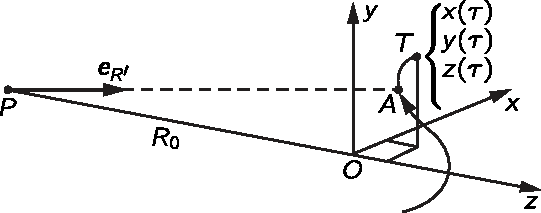
\includegraphics[width=0.9\linewidth]{fyz_fig0503.pdf}
    \caption{
             (\cite[s.~697]{Feynman01})}
    \label{fyz:fig0503}
  \end{figure}

  \begin{figure}[ht!] %\ref{fyz:fig0504}
    \centering
    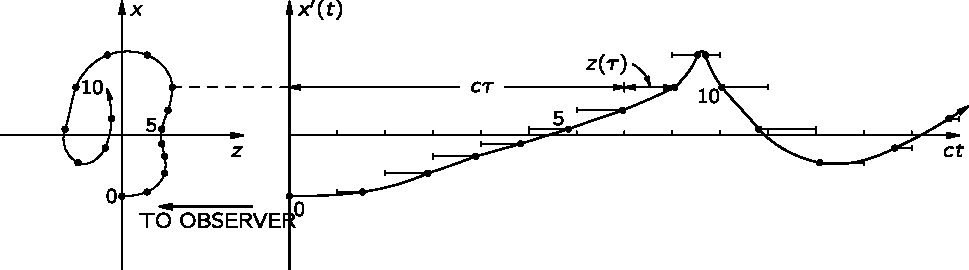
\includegraphics[width=1\linewidth]{fyz_fig0504.pdf}
    \caption{
             (\cite[s.~697]{Feynman01})}
    \label{fyz:fig0504}
  \end{figure}

  \begin{figure}[ht!] %\ref{fyz:fig0505}
    \centering
    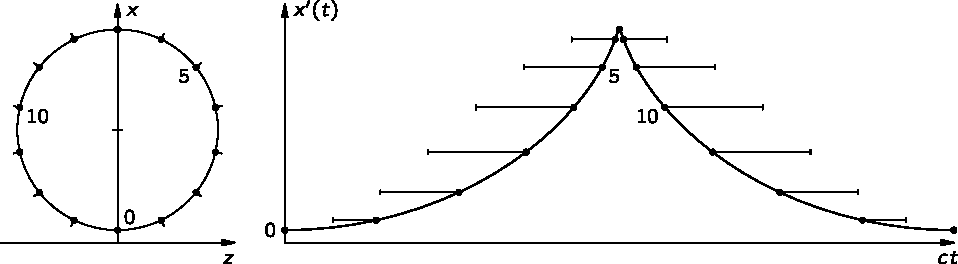
\includegraphics[width=1\linewidth]{fyz_fig0505.pdf}
    \caption{
             (\cite[s.~697]{Feynman01})}
    \label{fyz:fig0505}
  \end{figure}
  
  \begin{figure}[ht!] %\ref{fyz:fig0506}
    \centering
    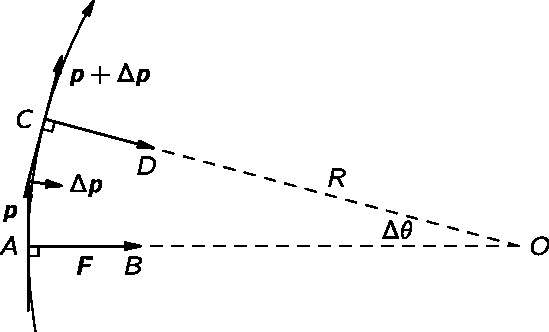
\includegraphics[width=0.9\linewidth]{fyz_fig0506.pdf}
    \caption{
             (\cite[s.~697]{Feynman01})}
    \label{fyz:fig0506}
  \end{figure}

  \begin{figure}[ht!] %\ref{fyz:fig0507}
    \centering
    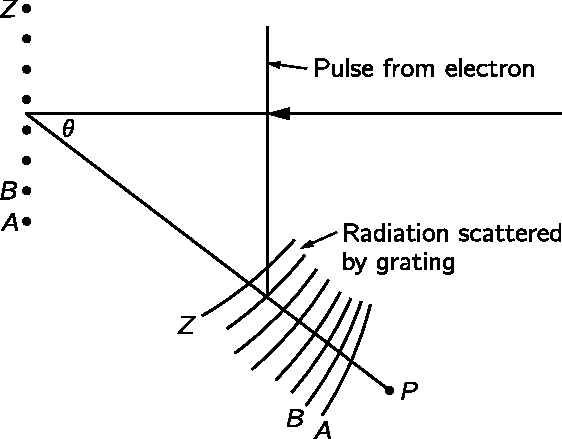
\includegraphics[width=0.9\linewidth]{fyz_fig0507.pdf}
    \caption{
             (\cite[s.~697]{Feynman01})}
    \label{fyz:fig0507}
  \end{figure}

  \begin{figure}[hb!] %\ref{fyz:fig0508}
    \centering
    \subcaptionbox{\label{fyz:fig0508a}}{\luafigure[0.8]{fyz_fig0508a.pdf}}
    \subcaptionbox{\label{fyz:fig0508b}}{\luafigure[0.8]{fyz_fig0508b.pdf}}
    \caption{
             (\cite[s.~601]{Feynman01}).}
    \label{fyz:fig0508}
  \end{figure}

  \begin{figure}[ht!] %\ref{fyz:fig0509}
    \centering
    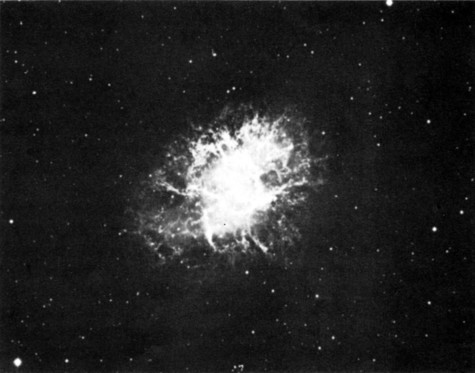
\includegraphics[width=0.6\linewidth]{fyz_fig0509.jpg}
    \caption{
             (\cite[s.~697]{Feynman01})}
    \label{fyz:fig0509}
  \end{figure}

  \begin{figure}[hb!] %\ref{fyz:fig0510}
    \centering
    \subcaptionbox{\label{fyz:fig0510a}}{\luafigure[0.8]{fyz_fig0510a.jpg}} \\
    \subcaptionbox{\label{fyz:fig0510b}}{\luafigure[0.8]{fyz_fig0510b.jpg}}  
    \caption{
             (\cite[s.~601]{Feynman01}).}
    \label{fyz:fig0510}
  \end{figure}

  \begin{figure}[hb!] %\ref{fyz:fig0511}
    \centering
    \subcaptionbox{\label{fyz:fig0511a}}{\luafigure[0.8]{fyz_fig0511a.pdf}} \\
    \subcaptionbox{\label{fyz:fig0511b}}{\luafigure[0.8]{fyz_fig0511b.pdf}}  
    \caption{
             (\cite[s.~601]{Feynman01}).}
    \label{fyz:fig0511}
  \end{figure}

  \begin{figure}[hb!] %\ref{fyz:fig0512}
    \centering
    \subcaptionbox{\label{fyz:fig0512a}}{\luafigure[0.8]{fyz_fig0512a.pdf}} \\
    \subcaptionbox{\label{fyz:fig0512b}}{\luafigure[0.8]{fyz_fig0512b.pdf}}  
    \caption{
             (\cite[s.~601]{Feynman01}).}
    \label{fyz:fig0512}
  \end{figure}

  \begin{figure}[ht!] %\ref{fyz:fig0513}
    \centering
    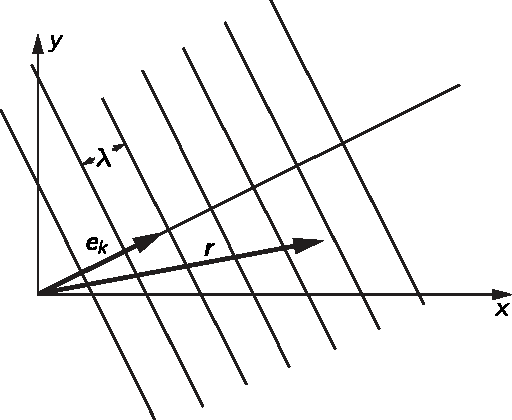
\includegraphics[width=0.8\linewidth]{fyz_fig0513.pdf}
    \caption{
             (\cite[s.~697]{Feynman01})}
    \label{fyz:fig0513}
  \end{figure}

  \begin{figure}[ht!] %\ref{fyz:fig0514}
    \centering
    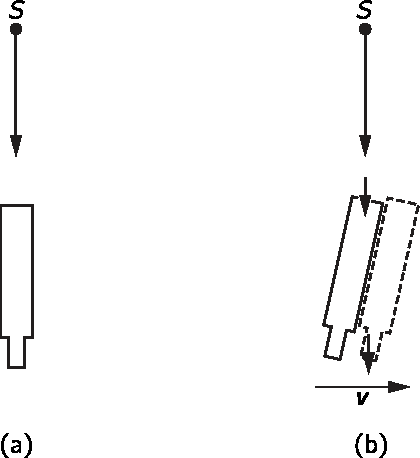
\includegraphics[width=0.7\linewidth]{fyz_fig0514.pdf}
    \caption{
             (\cite[s.~697]{Feynman01})}
    \label{fyz:fig0514}
  \end{figure}

  \begin{figure}[ht!] %\ref{fyz:fig0515}
    \centering
    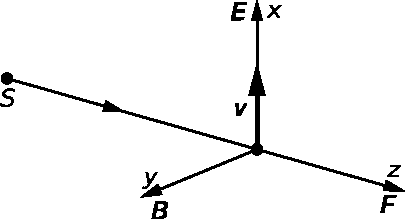
\includegraphics[width=0.6\linewidth]{fyz_fig0515.pdf}
    \caption{
             (\cite[s.~697]{Feynman01})}
    \label{fyz:fig0515}
  \end{figure}
 
  \todo[inline]{Kapitola fey1ch34 je zcela prázdná, pouze obrázky}    
%} %tikzset
%---------------------------------------------------------------------------------------------------